% ===================================================================
%  Week 4 — Session 2: Edge-preserving restoration & measuring quality
% ===================================================================
\documentclass[10pt,aspectratio=169]{beamer}
% ===================================================================
%  Shared Beamer preamble for "Practical Image Processing"
%  English slides. Compile with pdfLaTeX.
% ===================================================================

\usetheme{metropolis}
\usepackage[T1]{fontenc}
\usepackage[utf8]{inputenc}
\usepackage{lmodern}
\usepackage{listings}
\usepackage{tcolorbox}
\usepackage{fontawesome5}
\usepackage{booktabs}
\usepackage{amsmath,amssymb}
\usepackage{tikz}
\usepackage{pgfplots}
\pgfplotsset{compat=1.17}
\usetikzlibrary{arrows.meta,positioning,shapes.geometric,fit,backgrounds,matrix}
\tcbuselibrary{skins,breakable}

% ---- Palette --------------------------------------------------------
\definecolor{coursePrimary}{HTML}{1B4965}   % deep blue
\definecolor{courseAccent}{HTML}{E76F51}    % coral
\definecolor{courseGood}{HTML}{2A9D8F}      % teal
\definecolor{courseBad}{HTML}{C0392B}       % red
\definecolor{courseInfo}{HTML}{2980B9}      % blue
\definecolor{codeBg}{HTML}{F5F6FA}
\definecolor{codeKw}{HTML}{8E44AD}
\definecolor{codeStr}{HTML}{2A9D8F}
\definecolor{codeCom}{HTML}{7F8C8D}

\setbeamercolor{frametitle}{bg=coursePrimary}
\setbeamercolor{progress bar}{fg=courseAccent}
\setbeamercolor{alerted text}{fg=courseAccent}
\metroset{block=fill,sectionpage=progressbar,numbering=fraction}

% ---- Code listings (Python is built into listings) -----------------
\lstdefinestyle{course}{
  backgroundcolor=\color{codeBg},
  basicstyle=\ttfamily\scriptsize,
  keywordstyle=\color{codeKw}\bfseries,
  stringstyle=\color{codeStr},
  commentstyle=\color{codeCom}\itshape,
  numberstyle=\tiny\color{codeCom},
  numbers=left, numbersep=6pt,
  showstringspaces=false, breaklines=true, breakatwhitespace=true,
  tabsize=4, columns=fullflexible,
  frame=single, framesep=4pt, rulecolor=\color{gray!30},
  keepspaces=true, upquote=true, language=Python,
}
\lstset{style=course}
\lstdefinelanguage{bash}{
  keywords={cd,pip,python,venv,source,import}, sensitive=true,
  morecomment=[l]{\#}, morestring=[b]', morestring=[b]",
}

% ---- Reusable callout boxes ----------------------------------------
\newtcolorbox{goodbox}[1][Good practice]{colback=courseGood!8,colframe=courseGood,
  fonttitle=\bfseries,title={\faCheck~#1},boxrule=0.6pt,left=4pt,right=4pt,top=3pt,bottom=3pt}
\newtcolorbox{badbox}[1][Pitfall]{colback=courseBad!8,colframe=courseBad,
  fonttitle=\bfseries,title={\faTimes~#1},boxrule=0.6pt,left=4pt,right=4pt,top=3pt,bottom=3pt}
\newtcolorbox{infobox}[1][Note]{colback=courseInfo!8,colframe=courseInfo,
  fonttitle=\bfseries,title={\faInfoCircle~#1},boxrule=0.6pt,left=4pt,right=4pt,top=3pt,bottom=3pt}
\newtcolorbox{mathbox}[1][Math]{colback=coursePrimary!6,colframe=coursePrimary,
  fonttitle=\bfseries,title={\faCalculator~#1},boxrule=0.6pt,left=4pt,right=4pt,top=3pt,bottom=3pt}

\newcommand{\keyidea}[1]{\begin{alertblock}{Key idea}#1\end{alertblock}}
\newcommand{\term}[1]{\textbf{\color{coursePrimary}#1}}
\newcommand{\code}[1]{\lstinline[basicstyle=\ttfamily\small]|#1|}

% ---- A helper to draw a small pixel grid, cells shaded by value ----
% \pixelgrid{ {10,20,120,200,240}, {30,60,130,180,230}, ... }
\newcommand{\pixelgrid}[1]{%
  \begin{tikzpicture}[font=\scriptsize,scale=0.6]
    \foreach \row [count=\ry] in {#1} {
      \foreach \val [count=\cx] in \row {
        \draw[gray,fill=coursePrimary!8] (\cx,-\ry) rectangle ++(1,-1);
        \node at (\cx+0.5,-\ry-0.5) {\val};
      }
    }
  \end{tikzpicture}}


\title{Noise \& Restoration}
\subtitle{Week 4 — Session 2: Edge-preserving restoration \& measuring quality}
\author{Practical Image Processing}
\date{Lecture 4.2 \textbullet\ 60--70 min}

\begin{document}

\maketitle

\begin{frame}{Recap of Session 1}
  \begin{columns}[T]
    \begin{column}{0.58\textwidth}
      \begin{itemize}
        \item Noise \term{type} decides the cure: Gaussian/Poisson (grain) vs salt-and-pepper (specks).
        \item \term{Averaging} cuts Gaussian noise by $\sqrt{N}$ — but blurs edges.
        \item \term{Median} deletes impulses and keeps step edges — but can't help grain much.
        \item \alert{Today:} keep edges \emph{and} kill grain, handle hard cases, and \emph{measure} the result.
      \end{itemize}
    \end{column}
    \begin{column}{0.42\textwidth}
      \begin{alertblock}{The open problem}
        Plain averaging forces a choice: smooth flats \emph{or} keep edges. Can we have both?
      \end{alertblock}
    \end{column}
  \end{columns}
\end{frame}

\begin{frame}{Roadmap}\tableofcontents\end{frame}

% ==================================================================
\section{Edge-preserving filters}
% ==================================================================

\begin{frame}{The problem with plain averaging}
  \begin{itemize}
    \item A box/Gaussian kernel averages \emph{every} neighbour — including the ones on the \emph{other} side of an edge.
    \item So a sharp digit stroke on a light background gets a gray halo: the edge is blurred.
    \item Fix: average a neighbour \emph{only if} it really belongs to the same region.
  \end{itemize}
  \begin{center}
  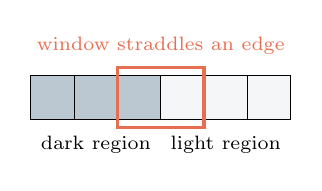
\begin{tikzpicture}[font=\scriptsize,scale=0.55]
    \foreach \x in {0,1,2} \draw[fill=coursePrimary!30] (\x,0) rectangle ++(1,1);
    \foreach \x in {3,4,5} \draw[fill=coursePrimary!5] (\x,0) rectangle ++(1,1);
    \draw[courseAccent,very thick] (2,-0.2) rectangle (4,1.2);
    \node[courseAccent] at (3,1.7) {window straddles an edge};
    \node at (1.5,-0.6) {\scriptsize dark region};
    \node at (4.5,-0.6) {\scriptsize light region};
  \end{tikzpicture}
  \end{center}
\end{frame}

\begin{frame}{The bilateral filter}
  \begin{columns}[T]
    \begin{column}{0.45\textwidth}\begin{center}
      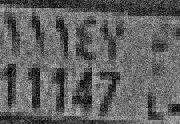
\includegraphics[width=0.85\linewidth]{../assets/gaussian_noise.png}\\{\scriptsize noisy}\\[4pt]
      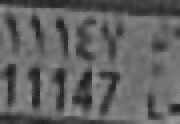
\includegraphics[width=0.85\linewidth]{../assets/gauss_denoise_bilateral.png}\\{\scriptsize bilateral}
    \end{center}\end{column}
    \begin{column}{0.55\textwidth}
      \begin{itemize}
        \item Weight each neighbour by \emph{two} things: how \term{close} it is (space) \emph{and} how \term{similar} its intensity is (range).
        \item Neighbours across an edge are far in \emph{intensity} $\rightarrow$ they get almost zero weight.
        \item Result: flats are smoothed, edges are preserved.
      \end{itemize}
      \begin{goodbox}
        For DocScan: bilateral before thresholding keeps digit edges crisp while killing sensor grain.
      \end{goodbox}
    \end{column}
  \end{columns}
\end{frame}

\begin{frame}{Bilateral filter — the math}
  \begin{mathbox}
    $\displaystyle g(p)=\frac{1}{W_p}\sum_{q\in\Omega}
      \underbrace{G_{\sigma_s}(\|p-q\|)}_{\text{spatial}}\;
      \underbrace{G_{\sigma_r}(|I(p)-I(q)|)}_{\text{range}}\;I(q)$
  \end{mathbox}
  \begin{itemize}
    \item $\sigma_s$: how far in \emph{space} we look; $\sigma_r$: how different in \emph{intensity} we still average.
    \item Small $\sigma_r \rightarrow$ only near-identical pixels count $\rightarrow$ strong edge preservation.
    \item Large $\sigma_r \rightarrow$ behaves like an ordinary Gaussian blur (edges blur again).
  \end{itemize}
  \begin{infobox}
    Two knobs, two jobs: $\sigma_s$ controls \emph{reach}, $\sigma_r$ controls \emph{edge sensitivity}.
  \end{infobox}
\end{frame}

\begin{frame}{Non-local means (NLM)}
  \begin{columns}[T]
    \begin{column}{0.45\textwidth}\begin{center}
      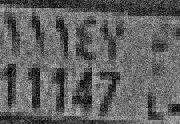
\includegraphics[width=0.85\linewidth]{../assets/gaussian_noise.png}\\{\scriptsize noisy}\\[4pt]
      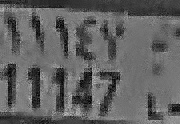
\includegraphics[width=0.85\linewidth]{../assets/gauss_denoise_nlm.png}\\{\scriptsize non-local means}
    \end{center}\end{column}
    \begin{column}{0.55\textwidth}
      \begin{itemize}
        \item Idea: average pixels whose surrounding \emph{patch} looks similar — even if they are far apart.
        \item An image repeats itself (many similar textures, strokes, flats); NLM exploits that redundancy.
        \item Best quality on Gaussian noise, at a real speed cost.
      \end{itemize}
      \keyidea{Bilateral compares single pixels; NLM compares whole neighbourhood \emph{patterns} — more robust.}
    \end{column}
  \end{columns}
\end{frame}

\begin{frame}{NLM: comparing patches, not pixels}
  \begin{center}
  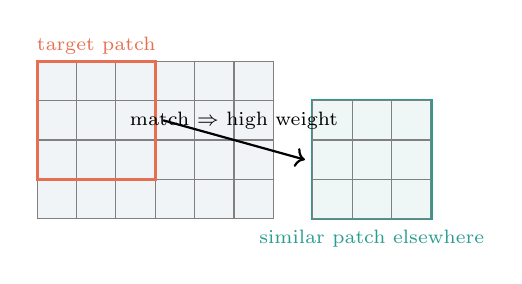
\begin{tikzpicture}[font=\scriptsize,scale=0.5]
    \foreach \x in {0,...,5}\foreach \y in {0,...,3}
      \draw[gray,fill=coursePrimary!6] (\x,\y) rectangle ++(1,1);
    \draw[courseAccent,very thick] (0,1) rectangle (3,4);
    \node[courseAccent] at (1.5,4.4) {target patch};
    \draw[courseGood,very thick] (7,0) rectangle (10,3);
    \foreach \x in {7,...,9}\foreach \y in {0,...,2}
      \draw[gray,fill=courseGood!8] (\x,\y) rectangle ++(1,1);
    \node[courseGood] at (8.5,-0.5) {similar patch elsewhere};
    \draw[->,thick] (3.2,2.5) -- (6.8,1.5) node[midway,above]{match $\Rightarrow$ high weight};
  \end{tikzpicture}
  \end{center}
  \begin{itemize}
    \item Weight $\propto \exp\!\big(-\|P(p)-P(q)\|^2/h^2\big)$ where $P(\cdot)$ is a small patch around a pixel.
    \item Larger $h$ = stronger denoising = more risk of washing out fine detail.
  \end{itemize}
\end{frame}

\begin{frame}{Bilateral vs NLM — how to choose}
  \begin{center}
  \begin{tabular}{@{}lll@{}}
    \toprule
    & \textbf{Bilateral} & \textbf{Non-local means} \\
    \midrule
    Compares & single pixel intensity & whole patch pattern \\
    Search area & local window & (semi-)global \\
    Speed & fast & slow \\
    Quality on grain & good & best \\
    Best for & real-time / edges & offline / max quality \\
    \bottomrule
  \end{tabular}
  \end{center}
  \begin{goodbox}
    Reach for bilateral when you need speed and crisp edges; reach for NLM when quality is worth the wait.
  \end{goodbox}
\end{frame}

\begin{frame}[fragile]{Edge-preserving filters in code}
\begin{lstlisting}[language=Python]
import cv2
# bilateral: d=9 window, sigmaColor=60 (range), sigmaSpace=60 (spatial)
bilateral = cv2.bilateralFilter(noisy, 9, 60, 60)

# non-local means: h=15 strength, templateWindow=7, searchWindow=21
nlm = cv2.fastNlMeansDenoising(noisy, None, 15, 7, 21)
\end{lstlisting}
  \begin{infobox}
    Bigger \code{sigmaColor}/\code{h} = stronger denoising but more lost detail. Tune on \emph{your} hard images, then measure.
  \end{infobox}
\end{frame}

% ==================================================================
\section{Adaptive \& order-statistic filters}
% ==================================================================

\begin{frame}{The order-statistic family}
  \begin{itemize}
    \item These filters \term{rank} the window's values and pick one — no averaging at all.
    \item \term{Median} = middle rank; \term{min} filter = rank 1 (removes salt); \term{max} filter = top rank (removes pepper).
    \item Because they return a \emph{real} pixel value, they never invent gray blends across edges.
  \end{itemize}
  \begin{mathbox}
    Sort the window $\{x_{(1)}\le\dots\le x_{(N)}\}$: \quad
    $\min=x_{(1)},\quad \text{median}=x_{((N+1)/2)},\quad \max=x_{(N)}.$
  \end{mathbox}
\end{frame}

\begin{frame}{Adaptive median filter}
  \begin{itemize}
    \item Plain median with a big window blurs; with a small window it misses dense impulse noise.
    \item \term{Adaptive median}: start small; \emph{grow} the window only where the centre still looks like an impulse.
    \item Cleans heavy salt-and-pepper while leaving clean regions almost untouched.
  \end{itemize}
  \begin{goodbox}
    For very noisy meter scans, an adaptive median can save digits a fixed median would smear.
  \end{goodbox}
\end{frame}

\begin{frame}{Worked: adaptive median in action}
  A pixel sits in heavy pepper; the $3\times3$ window is mostly \textbf{0}s:
  \begin{center}\pixelgrid{ {0,0,131}, {0,0,0}, {128,0,0} }\end{center}
  \begin{enumerate}
    \item $3\times3$ median $= 0$ — but 0 is itself an impulse, so \emph{don't} trust it: grow the window.
    \item At $5\times5$ enough true pixels ($\approx128\text{--}131$) appear; the median lands near \textbf{130}.
    \item Output \textbf{130} — a real gray, not a pepper dot. Fixed median would have output 0.
  \end{enumerate}
\end{frame}

% ==================================================================
\section{Temporal denoising}
% ==================================================================

\begin{frame}{Temporal denoising: average many frames}
  \begin{itemize}
    \item If you have several shots of the \emph{same} static scene, average them: noise cancels, signal stays.
    \item $N$ frames reduce Gaussian noise by $\sqrt{N}$ — the cheapest, highest-quality denoiser, with \emph{zero} blur.
    \item For a meter you can photograph twice, this beats any single-image filter.
  \end{itemize}
  \begin{goodbox}
    When you control capture, averaging a burst is the best denoising you can do — no detail lost.
  \end{goodbox}
\end{frame}

\begin{frame}{Worked: how many frames?}
  \begin{mathbox}
    $\sigma_{\text{out}}=\dfrac{\sigma}{\sqrt{N}}\;\Rightarrow\; N=\left(\dfrac{\sigma}{\sigma_{\text{target}}}\right)^{2}.$
  \end{mathbox}
  \begin{itemize}
    \item Grain has $\sigma=12$; you want it down to $\sigma_{\text{target}}=4$: $N=(12/4)^2=9$ frames.
    \item Want $\sigma=2$ instead? $N=(12/2)^2=36$ frames — quadratic cost for each halving.
    \item Unlike spatial filters, this costs \emph{no} sharpness — only capture time and a steady hand.
  \end{itemize}
  \begin{badbox}
    The scene must be \emph{static} and aligned. Any motion between frames turns averaging into motion blur.
  \end{badbox}
\end{frame}

% ==================================================================
\section{Measuring restoration}
% ==================================================================

\begin{frame}{Restoration vs enhancement}
  \begin{itemize}
    \item \term{Enhancement} (Wk2) makes an image \emph{look} better (subjective, no ground truth needed).
    \item \term{Restoration} tries to \emph{recover} the original by modelling the degradation (objective).
    \item Because restoration has a target, we can put a \emph{number} on success — that is what PSNR/SSIM do.
  \end{itemize}
  \keyidea{If you have a clean reference (or a synthetic-noise experiment), \emph{measure} — never just eyeball.}
\end{frame}

\begin{frame}{PSNR — peak signal-to-noise ratio}
  \begin{mathbox}
    $\mathrm{MSE}=\dfrac{1}{MN}\sum_{x,y}\big(f(x,y)-\hat f(x,y)\big)^2,\qquad
     \mathrm{PSNR}=10\log_{10}\dfrac{255^2}{\mathrm{MSE}}\;\text{dB}.$
  \end{mathbox}
  \begin{itemize}
    \item Compares your result $\hat f$ to a clean reference $f$; higher dB = closer.
    \item Rough guide: $>40$ dB excellent, $30\text{--}40$ good, $<30$ visible degradation.
    \item Simple and standard — but it only counts \emph{pixel} errors, not whether structure survived.
  \end{itemize}
\end{frame}

\begin{frame}{Worked: compute a PSNR}
  \begin{itemize}
    \item Suppose after denoising the mean-squared error vs the clean image is $\mathrm{MSE}=25$.
    \item $\mathrm{PSNR}=10\log_{10}\dfrac{255^2}{25}=10\log_{10}(2601)\approx 10\times3.415=\mathbf{34.1}$ dB.
    \item Halve the error to $\mathrm{MSE}=12.5$: PSNR rises about $3$ dB to $\approx 37.1$ dB (every $\times2$ in MSE $\approx 3$ dB).
  \end{itemize}
  \begin{infobox}
    Because it is logarithmic, small dB gains matter: $+3$ dB means you \emph{halved} the squared error.
  \end{infobox}
\end{frame}

\begin{frame}{SSIM — structural similarity}
  \begin{itemize}
    \item \term{SSIM} compares \emph{structure} (local luminance, contrast, correlation), not raw pixel error.
    \item Ranges $0$ to $1$; $1$ = identical. Matches human judgement far better than PSNR.
    \item A denoiser can win on PSNR yet lose on SSIM if it smears the very edges you care about.
  \end{itemize}
  \begin{goodbox}
    Report \emph{both}: PSNR for the error magnitude, SSIM for whether the digits' structure survived.
  \end{goodbox}
\end{frame}

\begin{frame}{The denoising dilemma}
  \begin{itemize}
    \item Every denoiser trades \term{noise removal} against \term{detail preservation}.
    \item Remove too little $\rightarrow$ noise breaks the next stage; too much $\rightarrow$ you erase the digits.
    \item There is no free lunch: choose the operating point for \emph{your} goal (readable digits).
  \end{itemize}
  \keyidea{Denoise for the downstream task, measured on hard images — not for the prettiest flat wall.}
\end{frame}

% ==================================================================
\section{Deblurring \& practice}
% ==================================================================

\begin{frame}{Deblurring \& the PSF}
  \begin{itemize}
    \item Blur = convolution with a \term{point-spread function} (PSF). Deblur = deconvolution.
    \item If you \emph{know} the PSF (motion length, defocus radius), you can partly invert it.
    \item Real methods regularize: \term{Wiener} (frequency-domain, noise-aware), \term{Richardson--Lucy} (iterative).
  \end{itemize}
  \begin{mathbox}
    Degradation model: $g = h * f + n$. Naive inverse $\hat f = g / H$ divides by the PSF spectrum — dangerous where $H\!\approx\!0$.
  \end{mathbox}
\end{frame}

\begin{frame}{Why naive deconvolution explodes}
  \begin{itemize}
    \item Where the PSF spectrum $H$ is near zero, dividing by it \emph{amplifies} any noise there to huge values.
    \item The result is dominated by amplified grain and ringing — worse than the blurry input.
    \item Regularization (Wiener) damps those frequencies using the noise-to-signal ratio.
  \end{itemize}
  \begin{badbox}
    Perfect deblurring is impossible when information is truly lost. A steady, well-lit shot beats any deconvolution.
  \end{badbox}
\end{frame}

\begin{frame}{Where denoising sits in the pipeline}
  \begin{center}
  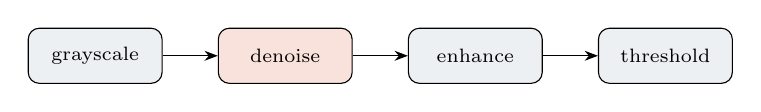
\begin{tikzpicture}[font=\scriptsize,>=Stealth,node distance=3mm and 7mm,
    b/.style={draw,rounded corners,fill=coursePrimary!8,minimum height=7mm,minimum width=17mm,align=center}]
    \node[b] (load){grayscale};
    \node[b,right=of load,fill=courseAccent!20] (den){denoise};
    \node[b,right=of den] (enh){enhance};
    \node[b,right=of enh] (thr){threshold};
    \draw[->](load)--(den);\draw[->](den)--(enh);\draw[->](enh)--(thr);
  \end{tikzpicture}
  \end{center}
  \begin{itemize}
    \item Denoise \emph{early} — before enhancement (which would amplify the noise) and before thresholding (which noise would corrupt).
    \item But not \emph{too} aggressively: over-denoising erases the digits you need.
  \end{itemize}
\end{frame}

\begin{frame}{Deep learning denoisers (preview)}
  \begin{itemize}
    \item Modern denoisers are CNNs trained on (noisy, clean) pairs — they beat classical methods on benchmarks.
    \item But they need data, compute, and can \emph{hallucinate} detail that isn't there.
    \item For DocScan, classical (median/bilateral/NLM) is usually enough and fully interpretable.
  \end{itemize}
  \begin{badbox}
    A hallucinated digit is worse than a noisy one — you cannot trust a reading you cannot audit.
  \end{badbox}
\end{frame}

\begin{frame}{\faPen~In-class exercise (10 min)}
  \begin{infobox}[Design \& measure a denoising experiment]
  \end{infobox}
  \begin{enumerate}
    \item You must keep digit edges razor-sharp while removing grain — which filter, and which two knobs do you tune?
    \item After denoising, $\mathrm{MSE}=6.5$ vs the clean image. Estimate the PSNR in dB.
    \item Your method scores high PSNR but low SSIM. What likely went wrong?
    \item You can capture 4 or 16 burst frames. How much does each cut the noise $\sigma$?
  \end{enumerate}
\end{frame}

\begin{frame}{\faPen~Debrief}
  \begin{itemize}
    \item (1) \term{Bilateral} (or NLM): tune $\sigma_s$ (reach) and $\sigma_r$ (edge sensitivity); keep $\sigma_r$ small.
    \item (2) $\mathrm{PSNR}=10\log_{10}(255^2/6.5)\approx\mathbf{40}$ dB — excellent.
    \item (3) It over-smoothed: pixel error is low but \emph{structure} (edges) was washed out — SSIM caught it.
    \item (4) $4$ frames $\rightarrow \sigma/2$; $16$ frames $\rightarrow \sigma/4$. Noise falls as $\sqrt{N}$.
  \end{itemize}
  \keyidea{Match the filter to the noise, then \emph{prove} it helped with a number on hard images.}
\end{frame}

% ==================================================================
\section{Wrap-up \& deliverable}
% ==================================================================

\begin{frame}{What you should now be able to do}
  \begin{itemize}
    \item Use edge-preserving filters (bilateral, NLM) and explain \emph{why} they keep edges.
    \item Reach for adaptive/order-statistic filters on heavy impulse noise, and temporal averaging when you control capture.
    \item Measure restoration with PSNR \emph{and} SSIM instead of eyeballing.
    \item Reason about deblurring's limits and place denoising correctly in the pipeline.
  \end{itemize}
\end{frame}

\begin{frame}{This week's deliverable}
  \begin{alertblock}{Due before Week 5 (see \code{project/})}
    \begin{enumerate}
      \item Add Gaussian and salt-pepper noise to a clean meter image (known noise = ground truth).
      \item Denoise each with 3 filters (e.g. median, bilateral, NLM); compute \term{PSNR} \emph{and} \term{SSIM} vs the clean original; tabulate.
      \item Show a case where the ``wrong'' filter fails (Gaussian on salt-pepper), and one where PSNR and SSIM \emph{disagree}.
      \item DocScan: denoise a real noisy meter photo so its Otsu/adaptive binary is clean and the digits stay sharp.
    \end{enumerate}
  \end{alertblock}
\end{frame}

\begin{frame}[standout]
  Keep the edges, kill the noise.\\[4pt]
  \normalsize Bilateral/NLM for grain, adaptive median for specks — and measure with PSNR + SSIM.
\end{frame}

\end{document}
